\scanpage{120}
\figure{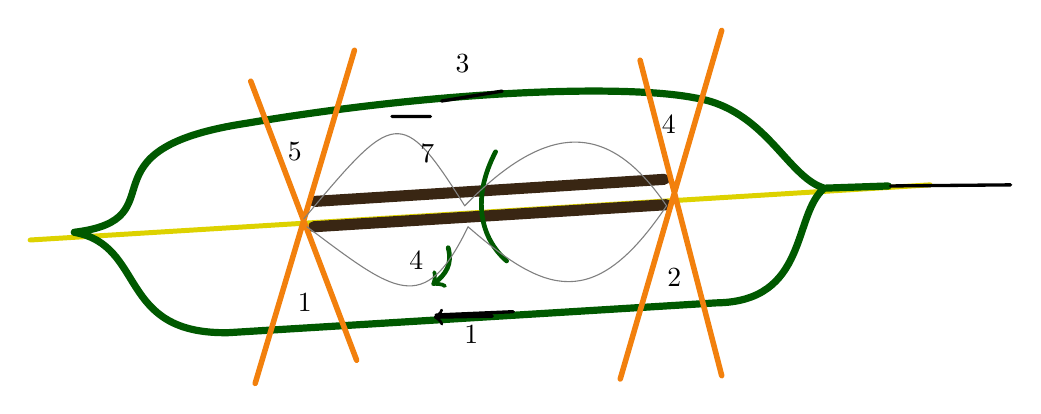
\begin{tikzpicture}[x=.014cm,y=-.014cm,line cap=round,line join=round]
\draw[yellow!70!olive,line width=1.8pt] (292,463)--(1108,413);
\draw[black!65!green,line width=2.6pt] (332,456)..controls(430,444)and(330,381)..(489,357)..controls(667,327)and(832,322)..(894,334)..controls(959,344)and(978,406)..(1012,416)--(1070,414) (332,456)..controls(398,468)and(370,549)..(472,547)--(914,520)..controls(998,519)and(983,440)..(1012,416);
\draw[black!70!brown,line width=4pt] (550,428)--(867,408) (549,451)--(869,431);
\draw[orange!80!brown,line width=2pt] (492,319)--(588,572) (586,291)--(496,593) (845,300)--(919,586) (919,273)--(827,589);
\draw[->,line width=1.2pt] (1072,414)--(1181,413) (665,337)--(720,328) (655,351)--(620,351) (660,531)--(730,528) (711,532)--(658,533);
\draw[black!65!green,line width=1.7pt,->] (714,383)..controls(692,425)and(700,461)..(724,482) (671,470)..controls(675,485)and(669,494)..(656,504);
\draw[gray] (540,444)..controls(622,346)and(628,340)..(686,432)..controls(763,353)and(818,357)..(869,432) (543,451)..controls(622,510)and(649,534)..(689,451)..controls(758,511)and(803,530)..(869,432);
\node at (532,383) {$5$};\node at (684,303) {$3$};\node at (871,358) {$4$};\node at (876,497) {$2$};\node at (541,520) {$1$};\node at (692,549) {$1$};\node at (652,385) {$\unsure{7}$};\node at (642,482) {$4$};
\end{tikzpicture}}

\figure{\begin{tikzpicture}[x=.018cm,y=-.018cm]
\draw[gray!65] (1408,382)--(1510,200)--(1591,396) (1464,304)--(1698,302) (1558,399)--(1695,193);
\fill[gray] (1564,304) circle(3);\node at (1544,290) {$1$};
\end{tikzpicture}}

\figure{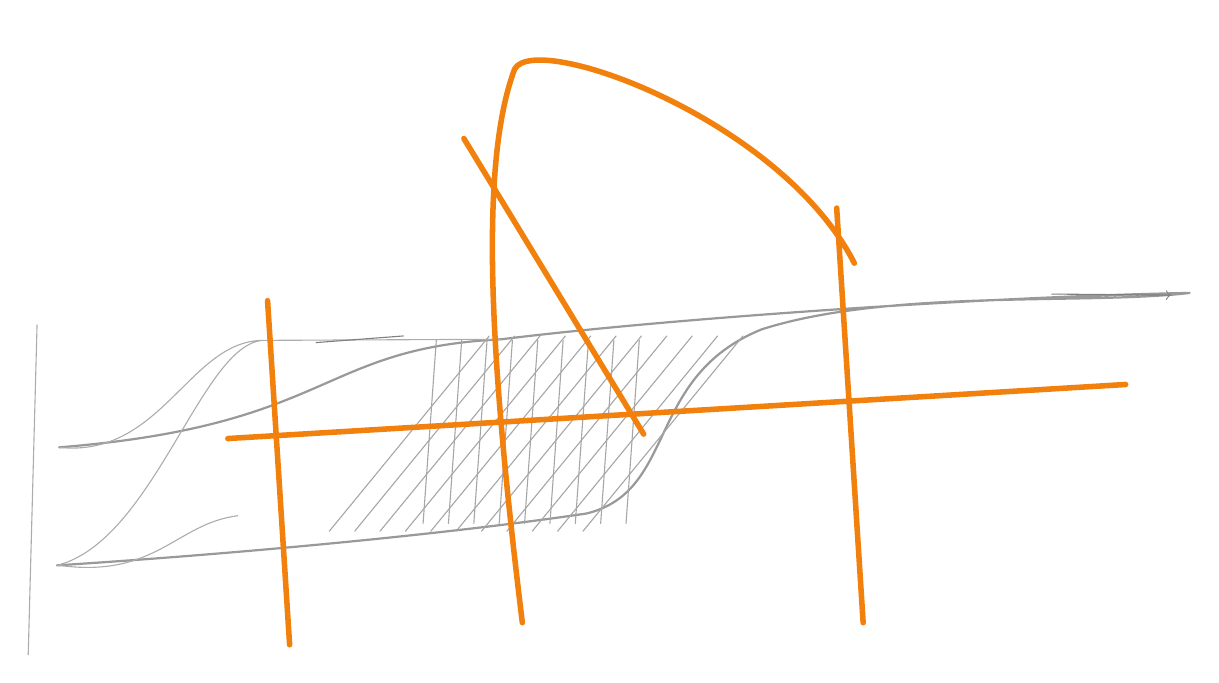
\begin{tikzpicture}[x=.014cm,y=-.014cm,line cap=round,line join=round]
\draw[gray!80,line width=.8pt] (150,968)..controls(398,948)and(385,878)..(551,870)..controls(713,850)and(1003,831)..(1175,828) (148,1075)..controls(349,1062)and(527,1043)..(628,1028)..controls(711,1008)and(681,904)..(787,861)..controls(903,824)and(1083,839)..(1175,828);
\draw[gray!65] (150,968)..controls(243,978)and(268,871)..(335,871)--(550,870) (148,1075)..controls(236,1053)and(279,874)..(335,871) (150,1075)..controls(238,1087)and(256,1037)..(312,1030) (122,1156)--(130,857);
\foreach \x in {395,418,...,626}\draw[gray!70] (\x,1044)--(\x+145,867);
\foreach \x in {480,503,...,686}\draw[gray!70] (\x,1037)--(\x+12,871);
\draw[orange!80!brown,line width=2pt] (339,835)--(359,1147) (303,960)--(1117,911) (517,688)--(680,956) (570,1127)..controls(544,914)and(528,718)..(563,625)..controls(582,590)and(805,671)..(871,801) (855,751)--(879,1127);
\draw[gray,->] (383,873)--(462,867) (1050,829)--(1158,830);
\end{tikzpicture}}

\figure{\begin{tikzpicture}[x=.011cm,y=-.011cm,line cap=round,line join=round]
\draw[gray!70] (1044,981)..controls(1120,893)and(1263,862)..(1369,962)..controls(1430,1088)and(1196,1124)..(1100,1083)..controls(1037,1060)and(1034,994)..(1044,981) (1050,977)..controls(1137,1006)and(1287,985)..(1369,962);
\draw[gray!75] (1354,1090)..controls(1390,913)and(1484,762)..(1554,618)..controls(1619,467)and(1675,417)..(1760,432)..controls(1915,459)and(1755,651)..(1680,790)..controls(1547,1005)and(1461,1181)..(1398,1165)..controls(1346,1148)and(1347,1122)..(1354,1090);
\draw[gray!65] (1367,1088)..controls(1418,893)and(1505,772)..(1564,622)..controls(1635,479)and(1681,425)..(1764,443)..controls(1900,471)and(1737,670)..(1660,801)..controls(1541,1006)and(1460,1166)..(1402,1154)..controls(1353,1143)and(1360,1125)..(1367,1088);
\foreach \x/\y in {1370/1110,1373/1127,1384/1142,1397/1153,1409/1136,1434/1080,1453/1048,1470/1018,1494/986,1510/950,1520/916,1550/868,1570/820,1597/770,1611/729,1627/685,1648/635,1663/597,1674/548}\draw[gray!70] (\x,\y)--++(118,-76);
\draw[gray!60] (1661,454)--(1787,747) (1578,554)--(1721,850) (1404,461)--(1592,810) (1691,608)--(1972,938) (1359,865)--(1741,857);
\draw[gray!65] (1091,1357)..controls(1063,1257)and(1149,1176)..(1209,1127)..controls(1334,1035)and(1369,1156)..(1437,1315)..controls(1459,1382)and(1350,1459)..(1244,1462)..controls(1176,1468)and(1090,1419)..(1091,1357) (1072,1319)..controls(1120,1281)and(1160,1279)..(1223,1254)..controls(1287,1224)and(1385,1271)..(1437,1315) (1223,1254)--(1219,1449) (1295,1164)--(1262,1445) (1351,1111)..controls(1347,1213)and(1379,1335)..(1417,1369);
\draw[line width=1.2pt] (1072,1319)--(1085,1365) (1175,1451)..controls(1203,1457)and(1230,1457)..(1262,1449) (1417,1369)--(1437,1323);
\node at (1329,1350) {$\ast$};
\draw[gray!55] (1013,1552)..controls(1055,1411)and(1156,1430)..(1205,1483)..controls(1361,1673)and(1215,1752)..(1109,1720)..controls(1040,1695)and(986,1633)..(1013,1552) (1060,1513)..controls(1100,1480)and(1136,1500)..(1162,1538);
\draw[gray!55] (2115,818)..controls(2155,661)and(2360,511)..(2441,590)..controls(2586,616)and(2649,872)..(2451,977)..controls(2323,1044)and(2103,1008)..(2115,818) (2264,1004)--(2441,590);
\fill[gray!70] (2441,590) circle(3);
\end{tikzpicture}}

\figure{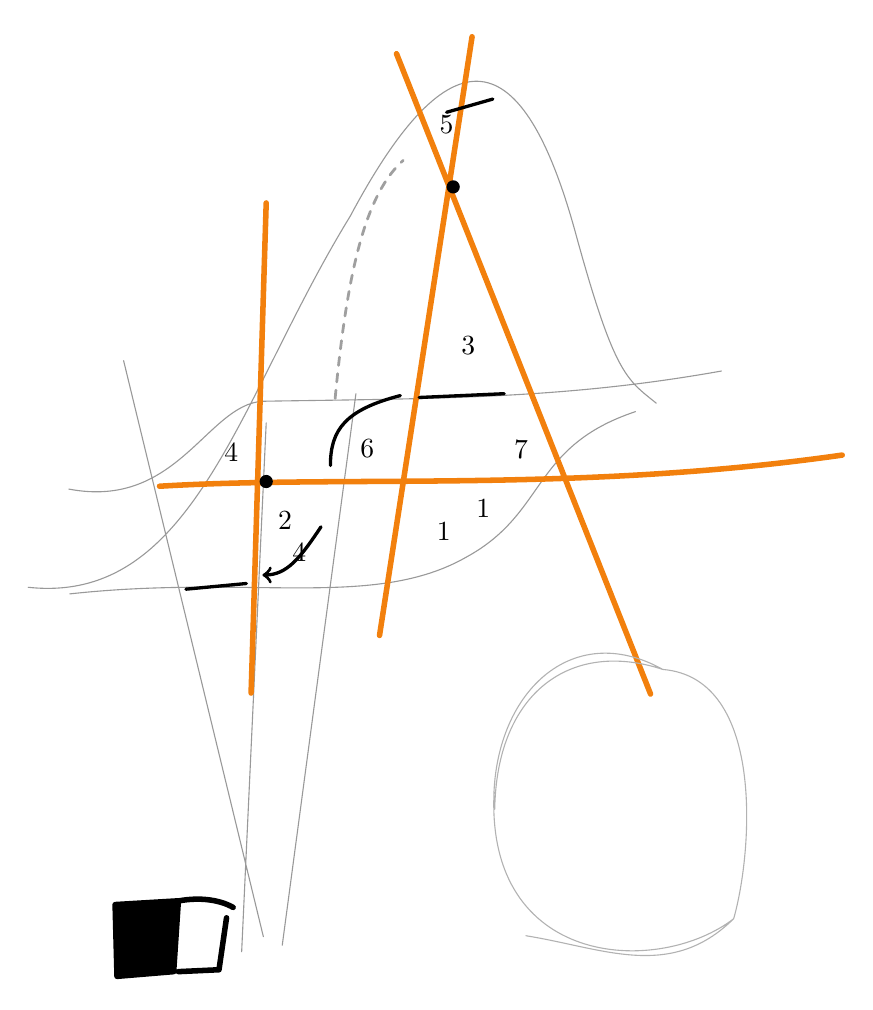
\begin{tikzpicture}[x=.012cm,y=-.012cm,line cap=round,line join=round]
\draw[gray!80] (260,1778)..controls(436,1797)and(483,1577)..(601,1385)..controls(707,1186)and(784,1196)..(841,1408)..controls(881,1553)and(894,1558)..(925,1583) (303,1674)..controls(418,1696)and(449,1585)..(508,1581)..controls(691,1578)and(826,1579)..(994,1549) (304,1785)..controls(496,1764)and(626,1802)..(724,1746)..controls(810,1699)and(792,1629)..(903,1592) (361,1538)--(509,2148) (512,1604)--(486,2164) (607,1573)--(529,2157);
\draw[gray!75,dashed,line width=1pt] (585,1578)..controls(598,1440)and(618,1361)..(657,1326);
\draw[orange!80!brown,line width=2pt] (512,1371)--(496,1890) (650,1213)--(919,1891) (730,1195)--(632,1829) (399,1671)..controls(596,1659)and(841,1678)..(1122,1638);
\fill (512,1666) circle(7) (710,1354) circle(7);
\draw[->,line width=1.2pt] (654,1575)..controls(596,1590)and(580,1611)..(580,1649) (703,1275)--(752,1261) (674,1577)--(764,1573) (491,1774)--(427,1780) (570,1714)..controls(548,1747)and(534,1765)..(508,1765);
\node at (475,1635) {$4$};\node at (532,1707) {$2$};\node at (619,1631) {$6$};\node at (726,1522) {$3$};\node at (782,1632) {$7$};\node at (700,1719) {$1$};\node at (742,1695) {$1$};\node at (703,1288) {$5$};\node at (547,1741) {$\unsure{4}$};
\draw[gray!60] (753,2005)..controls(753,1891)and(835,1811)..(932,1865)..controls(1041,1874)and(1027,2059)..(1007,2129)..controls(929,2189)and(751,2182)..(753,2005) (754,2013)..controls(756,1889)and(835,1833)..(932,1865) (787,2147)..controls(869,2160)and(940,2195)..(1007,2129);
\draw[line width=2pt] (352,2114)--(419,2110)--(414,2185)--(354,2190)--cycle (419,2185)--(462,2183)--(470,2128) (420,2110)..controls(442,2106)and(463,2109)..(477,2117);
\fill (354,2115)--(418,2110)--(414,2185)--(355,2190)--cycle;
\end{tikzpicture}}

\figure{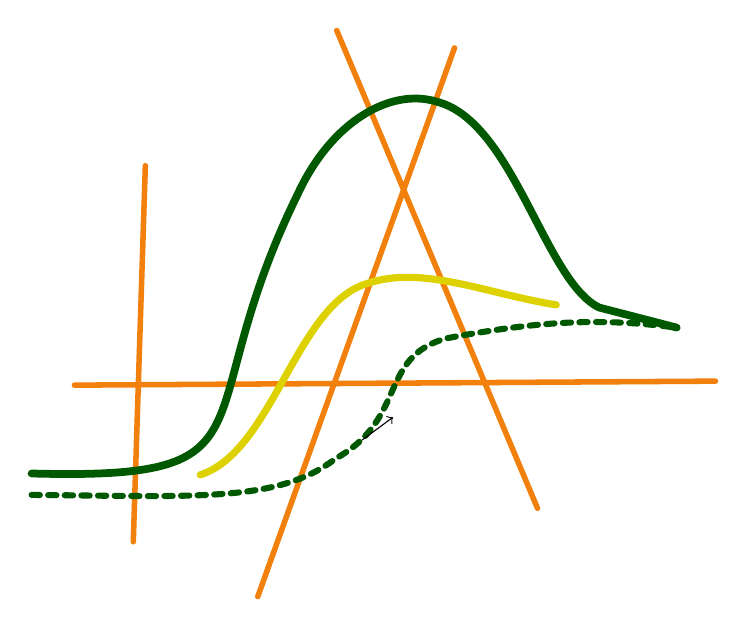
\begin{tikzpicture}[x=.017cm,y=-.017cm,line cap=round,line join=round]
\draw[orange!80!brown,line width=2pt] (1353,1547)--(1344,1828) (1496,1446)--(1646,1803) (1584,1459)--(1437,1869) (1300,1711)--(1779,1708);
\draw[black!65!green,line width=2.8pt] (1268,1777)..controls(1457,1782)and(1382,1741)..(1467,1568)..controls(1492,1514)and(1536,1489)..(1570,1499)..controls(1628,1513)and(1651,1633)..(1692,1653)--(1750,1668);
\draw[yellow!70!olive,line width=2.6pt] (1394,1778)..controls(1448,1761)and(1466,1650)..(1519,1635)..controls(1560,1621)and(1609,1643)..(1660,1651);
\draw[black!65!green,line width=2.2pt,dashed] (1268,1793)..controls(1390,1794)and(1452,1799)..(1495,1766)..controls(1549,1736)and(1527,1690)..(1578,1676)..controls(1642,1664)and(1689,1660)..(1750,1668);
\draw[->] (1515,1752)--(1538,1735);
\end{tikzpicture}}

\[
(n-2)\unsure{-|+}(n-3)=2n-5
\]
\[2(n-1)(2n-5)\qquad2n\]

\[
\chi(\unsure{\mathcal X|X})=s_0-s_1+s_2=1-g
\]
Les sommets sont d'ordre 4

On trouve donc
\[
2s_1=\underbrace{4s_0}_{\sum_{s\in S}\nu_s}=2\sum_{f\in F}n_f
\]
\deleted{$\unsure{s_2=}$}

donc $s_1=2s_0$

donc $\chi(\unsure{\mathcal X|X})=s_2-s_0\unsure{\Leftarrow|\Leftrightarrow}\qquad g=1+s_0-s_2$

où $s_2=$ nombre des p.r. (les \unsure{super-singuliers} exclus)

$s_0=$ nombre des sommets, i.e \deleted{de}

a) des couples $(D,a)$, où $D$ est une psdr. et $a$ un arc d'\unsure{inertie} \deleted{\unsure{compatible avec}} en $D$ de type gén-gén.

b) des \deleted{\unsure{1-points de type}} \inserted{\unsure{drapeaux de type}} de $\deleted{\unsure{\Sigma}}^{(0,1)}$ \inserted{de $\Sigma$} ($=2n(n-1)$ dans les cas stables)

\figure{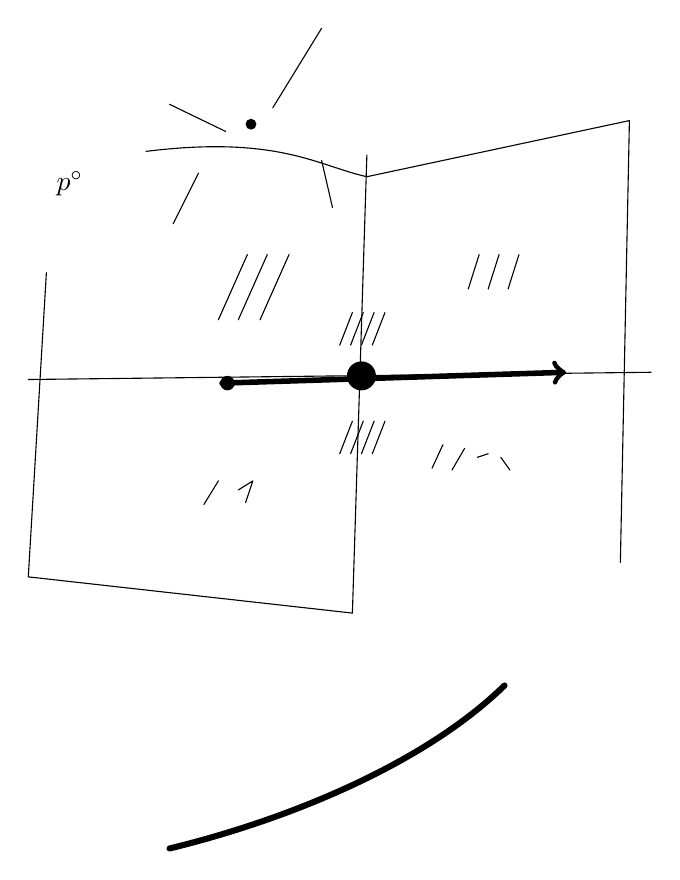
\begin{tikzpicture}[x=.023cm,y=-.023cm,line cap=round,line join=round]
\draw (2540,1057)--(2530,1225)--(2709,1245)--(2717,992) (2595,990)..controls(2668,981)and(2690,998)..(2717,1004)--(2862,973)--(2857,1217) (2530,1116)--(2874,1112);
\draw[line width=2pt,->] (2637,1118)--(2827,1112);\fill (2714,1114) circle(8) (2640,1118) circle(4) (2653,975) circle(3);
\draw (2608,964)--(2639,979) (2665,966)--(2692,922) (2624,1002)--(2610,1030) (2692,995)--(2698,1021);
\foreach \x in {2635,2646,2658}\draw (\x,1083)--++(16,-36);
\foreach \x in {2702,2708,2714,2720}\draw (\x,1097)--++(7,-18) (\x,1157)--++(7,-18);
\foreach \x in {2773,2784,2795}\draw (\x,1066)--++(6,-19);
\draw (2627,1185)--(2635,1172) (2646,1177)--(2654,1172)--(2650,1184) (2753,1165)--(2759,1152) (2764,1166)--(2771,1154) (2778,1159)--(2784,1157) (2791,1159)--(2796,1166);
\node at (2553,1008) {$\unsure{p^\circ}$};\draw[line width=2.2pt] (2608,1375)..controls(2674,1359)and(2749,1328)..(2793,1285);
\end{tikzpicture}}
\margin{119}
